\documentclass[hyperref={pdfpagelabels=false}]{beamer}
\usepackage{lmodern}
\title{Bisphenol-A}   
\author{Jakob Bolenbach} 
\date{\today} 
\setbeamertemplate{navigation symbols}{}
\usepackage{beamerthemeshadow}
\beamersetuncovermixins{\opaqueness<1>{25}}{\opaqueness<2->{15}}
\usepackage{natbib}                  
\usepackage{bibgerm} 

\begin{document}
\begin{frame}
\titlepage
\end{frame} 

\section{Was ist das?} 
\begin{frame}
\frametitle {Was ist das?}
\begin{figure}
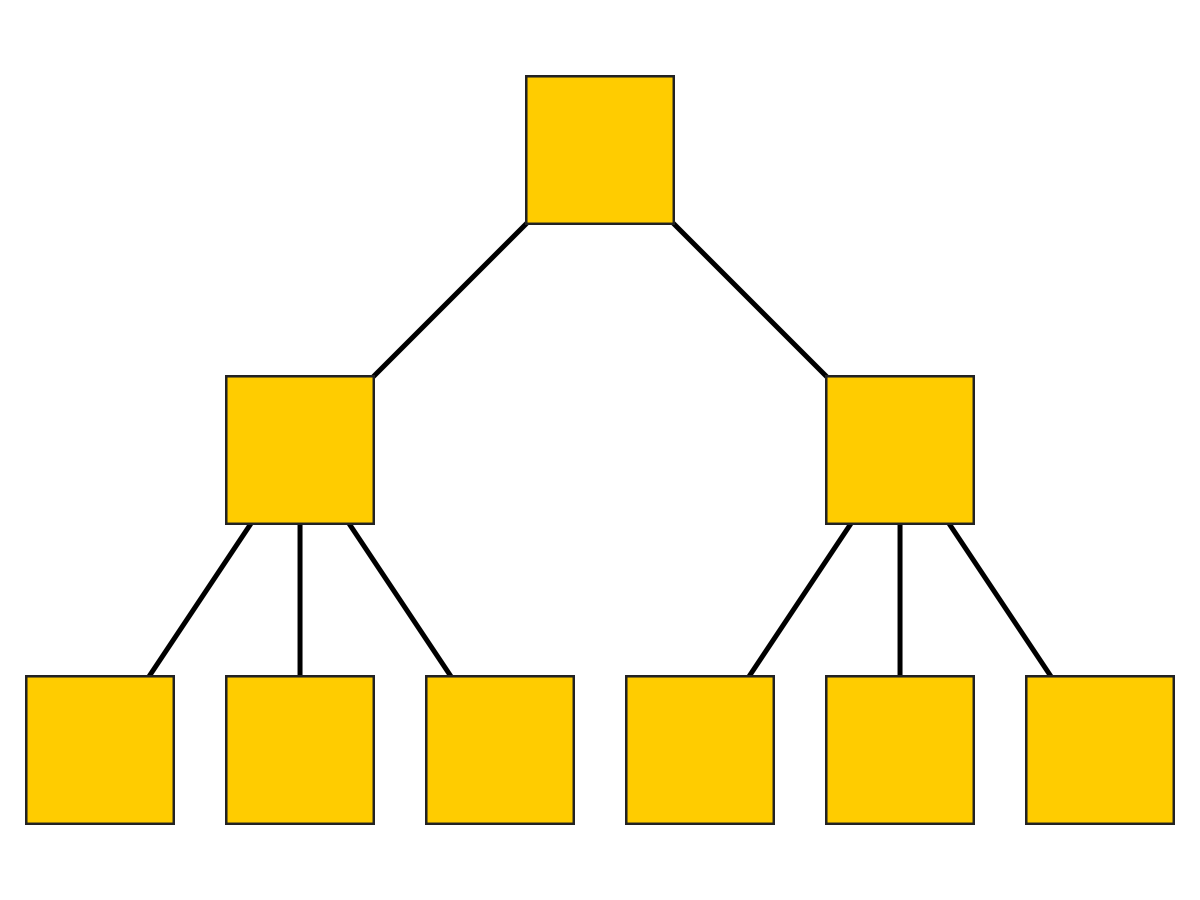
\includegraphics[scale=.2]{HD.png}
\centering
\end{figure}
\end{frame}

\section{Pro und Kontra} 
\subsection{Darstellung, Aufbau und Risiken}

\begin{frame}
\frametitle{Vor und Nachteile}
\begin{center}
\begin{table}
\scriptsize
\begin{tabular}{|c|c|}
\hline
Vorteile & Nachteile\\
\hline
\pause
Einfach & \pause Unflexibel\\
\hline
\pause
Einfacher Zugriff auf zusammenhängende Strukturen & \pause Zugriff nur durch die Hierarchie\\
\hline
\pause
Schneller Zugriff bei bekannten Pfaden & \pause Keine bidirektionalen Beziehungen\\
\hline
\end{tabular}
\end{table}
\end{center}
\end{frame}

\section{Beispiele} 
\begin{frame}
\frametitle{Beispiele}
\end{frame}

\section{Quellen}
\begin{frame}
\frametitle{Quellen}
\begin{enumerate} 
\item $https://www.softguide.de/software-tipps/hierarische-datenbanken$
\end{enumerate}
\end{frame}

\end{document}